\chapter{$\alpha_p$-Studie}

\section*{As-received-Proben (VR)}

Die Proben sind zylindrische Stangenabschnitte mit einem Durchmesser von 19 mm und einer Höhe von 8 mm. Der Zustand der Proben ist rekristallisationsgeglüht. Eine metallografische Untersuchung des Gefüges zeigt eine globulare Mikrostruktur mit einem $\alpha_p$-Volumenanteil von 62\%. 


\section{Durchführung (VR)}

Zur Maximierung der Zugfestigkeit der Legierung Ti-6242 wurde zuerst der Einfluss des $\alpha_p$-Phasenanteils auf die Härte untersucht. Laut Lütjering \cite{Lutjering.2007} konnte bei der Legierung IMI 834 eine maximale Zugfestigkeit bei einem $\alpha_p$-Anteil von 10--20\% festgestellt werden. \\
Um eine größtmögliche Härtesteigerung gegenüber der as-received-Probe (AR) zu erzielen, wurden vier Proben bei unterschiedlichen Temperaturen 1h unterhalb der $\beta$-Transus-Temperatur geglüht und anschließend luftgekühlt (AC: air cooled) (Tab. \ref{tab:alphap}). Zu erwarten sind abnehmende $\alpha_p$-Volumenanteile mit steigender Temperatur. Zusätzlich wurde eine Probe bei 1015$^\circ$C 30min lang geglüht und wassergekühlt, um ein vollmartensitisches Gefüge einzustellen. Die fünf Proben wurden inklusive einer AR-Probe metallografisch präpariert und ausgewertet.



\begin{table}[h]
	\centering
	\begin{tabular}{|c|c|c|c|}
		\hline 
		Probenbezeichnung & Temperatur [$^\circ$C] & Zeit [h] & Abkühlmethode \\ 
		\hline 
		BM990 & 990 & 1 & AC\\ 
		\hline 
		BM983 & 983 & 1 & AC\\
		\hline
		BM975 & 975 & 1 & AC\\ 
		\hline
		BM960 & 960 & 1 & AC\\ 
		\hline 
		M1015 & 1015 & 0.5 & WQ\\ 
		\hline
	\end{tabular} 
	\caption{Wärmebehandlungen der $\alpha_p$-Studie}
	\label{tab:alphap}
\end{table}



\section{Ergebnisse (PH)}

Im Rahmen der $\alpha_p$-Studie wurden zunächst vier Proben bei verschiedenen Temperaturen unterhalb der $\beta$-Transus-Temperatur (995$^\circ$C für Ti-6242) wärmebehandelt. Ziel war die Einstellung einer bi-modalen Mikrostruktur, sowie die Bestimmung des $\alpha_p$-Volumenanteils. Die Auswertung dieser Proben unter dem Lichtmikroskop ist in Abbildung \ref{fig:abbildung-8} aufgeführt. 

\begin{figure}[h]
	\centering
	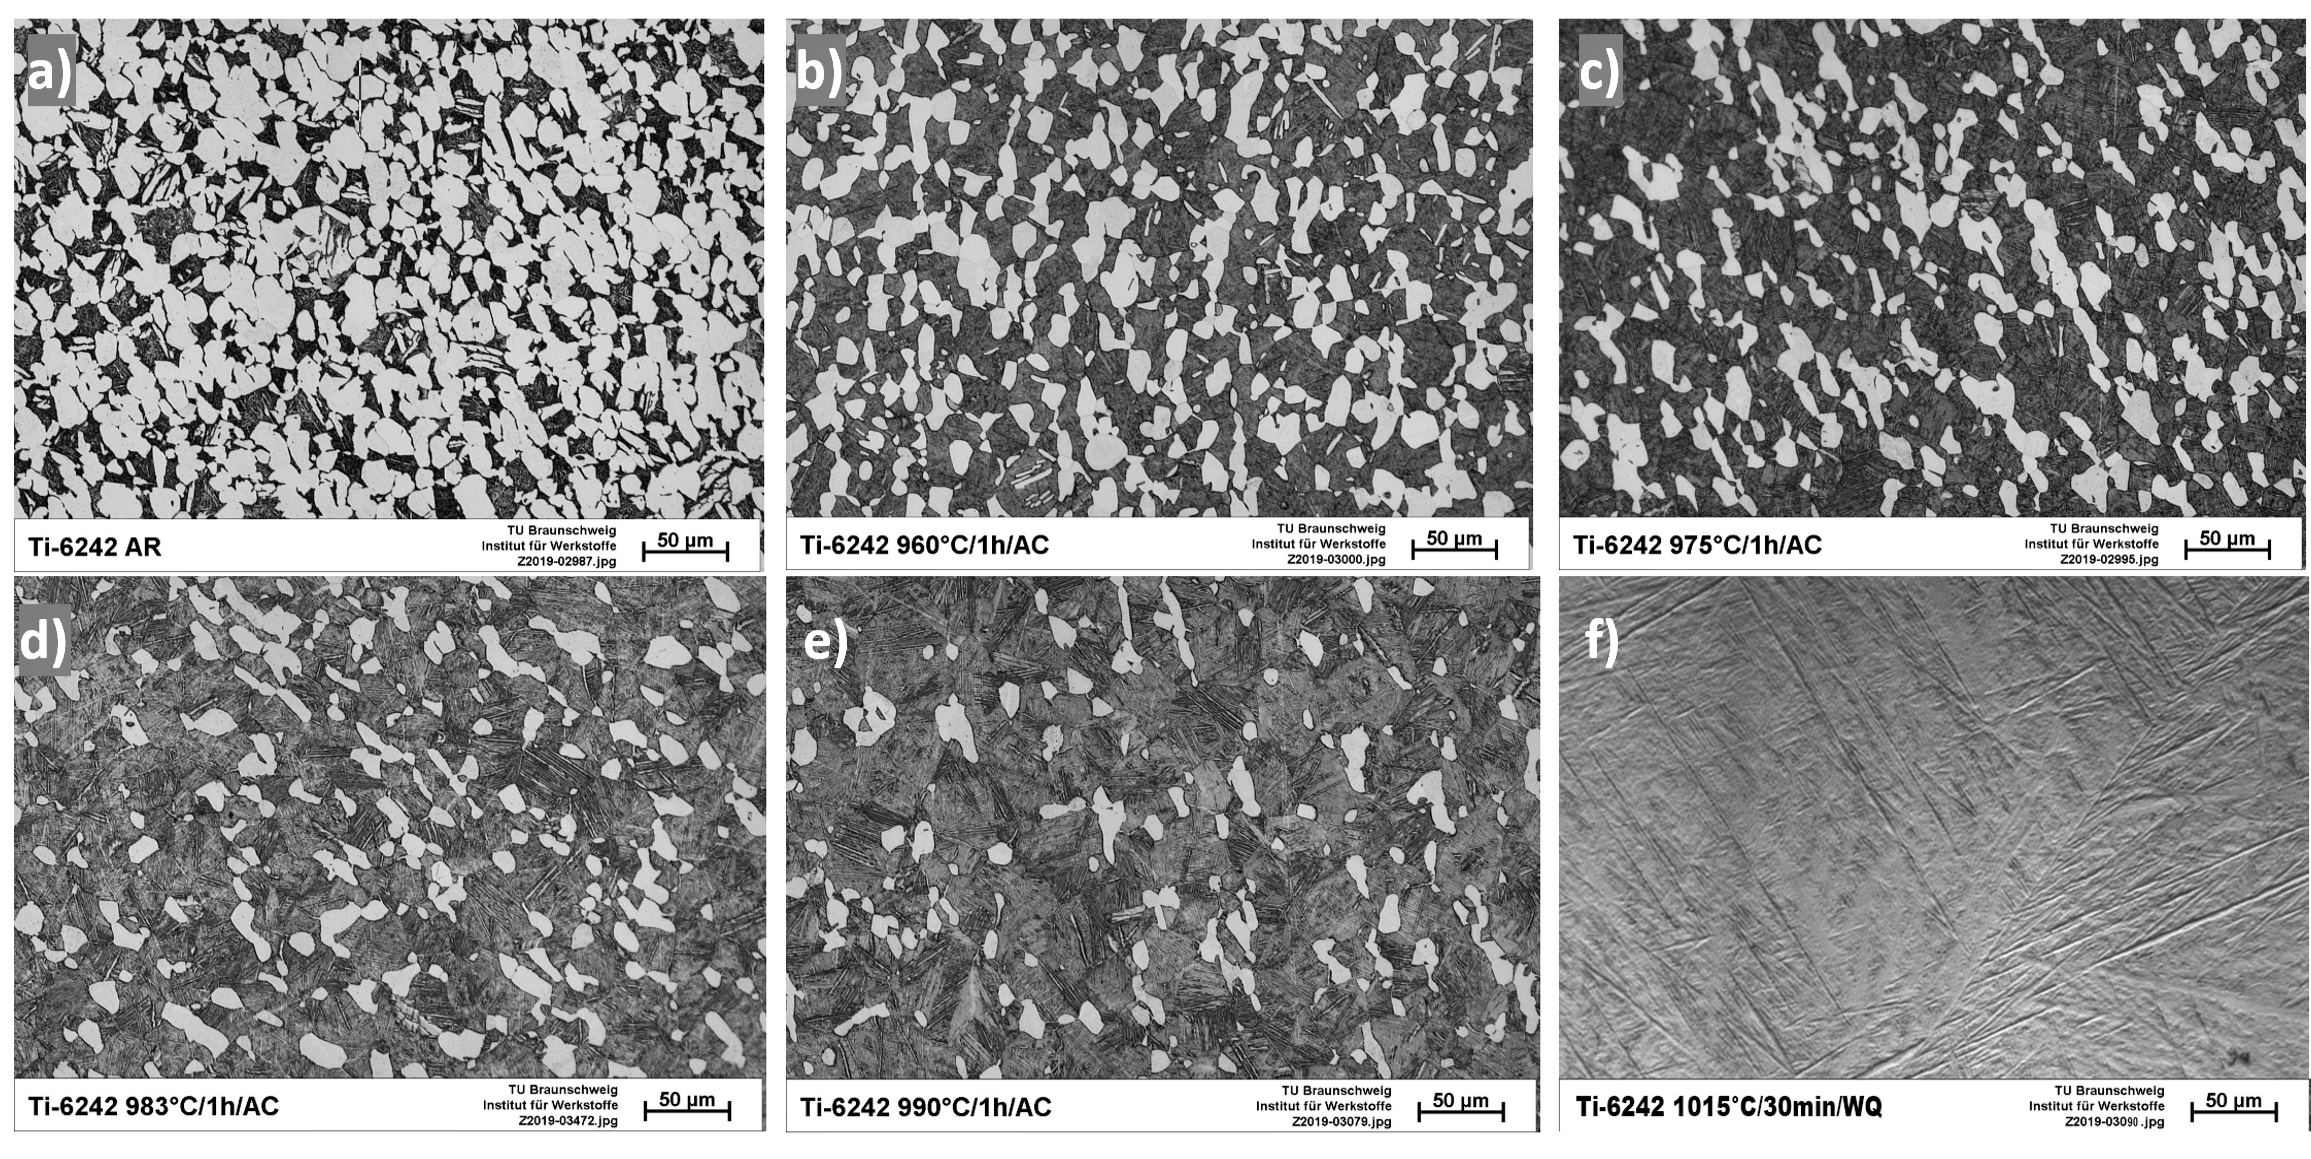
\includegraphics[width=1.0\linewidth]{./Bilder/Abbildung 8.png}
	\caption[Abbildung 8]{Mikrostrukturen der verwendeten Ti-6242 Legierung vor und nach der ersten Wärmebehandlung bei verschiedenen Temperaturen, a) Mikrostruktur vor Wärmebehandlung (AR), b) 960$^\circ$C/1h/AC, c) 975$^\circ$C/1h/AC, d) 983$^\circ$C/1h/AC, e) 990$^\circ$C/1h/AC, f) 1015$^\circ$C/30min/WQ vollmartensitisches Gefüge}
	\label{fig:abbildung-8}
\end{figure}

Ein Überblick über die in der bi-modalen Mikrostruktur auftretenden Gefügebestandteile zeigt die Abbildung \ref{fig:abbildung-20}.

\begin{figure}[h]
	\centering
	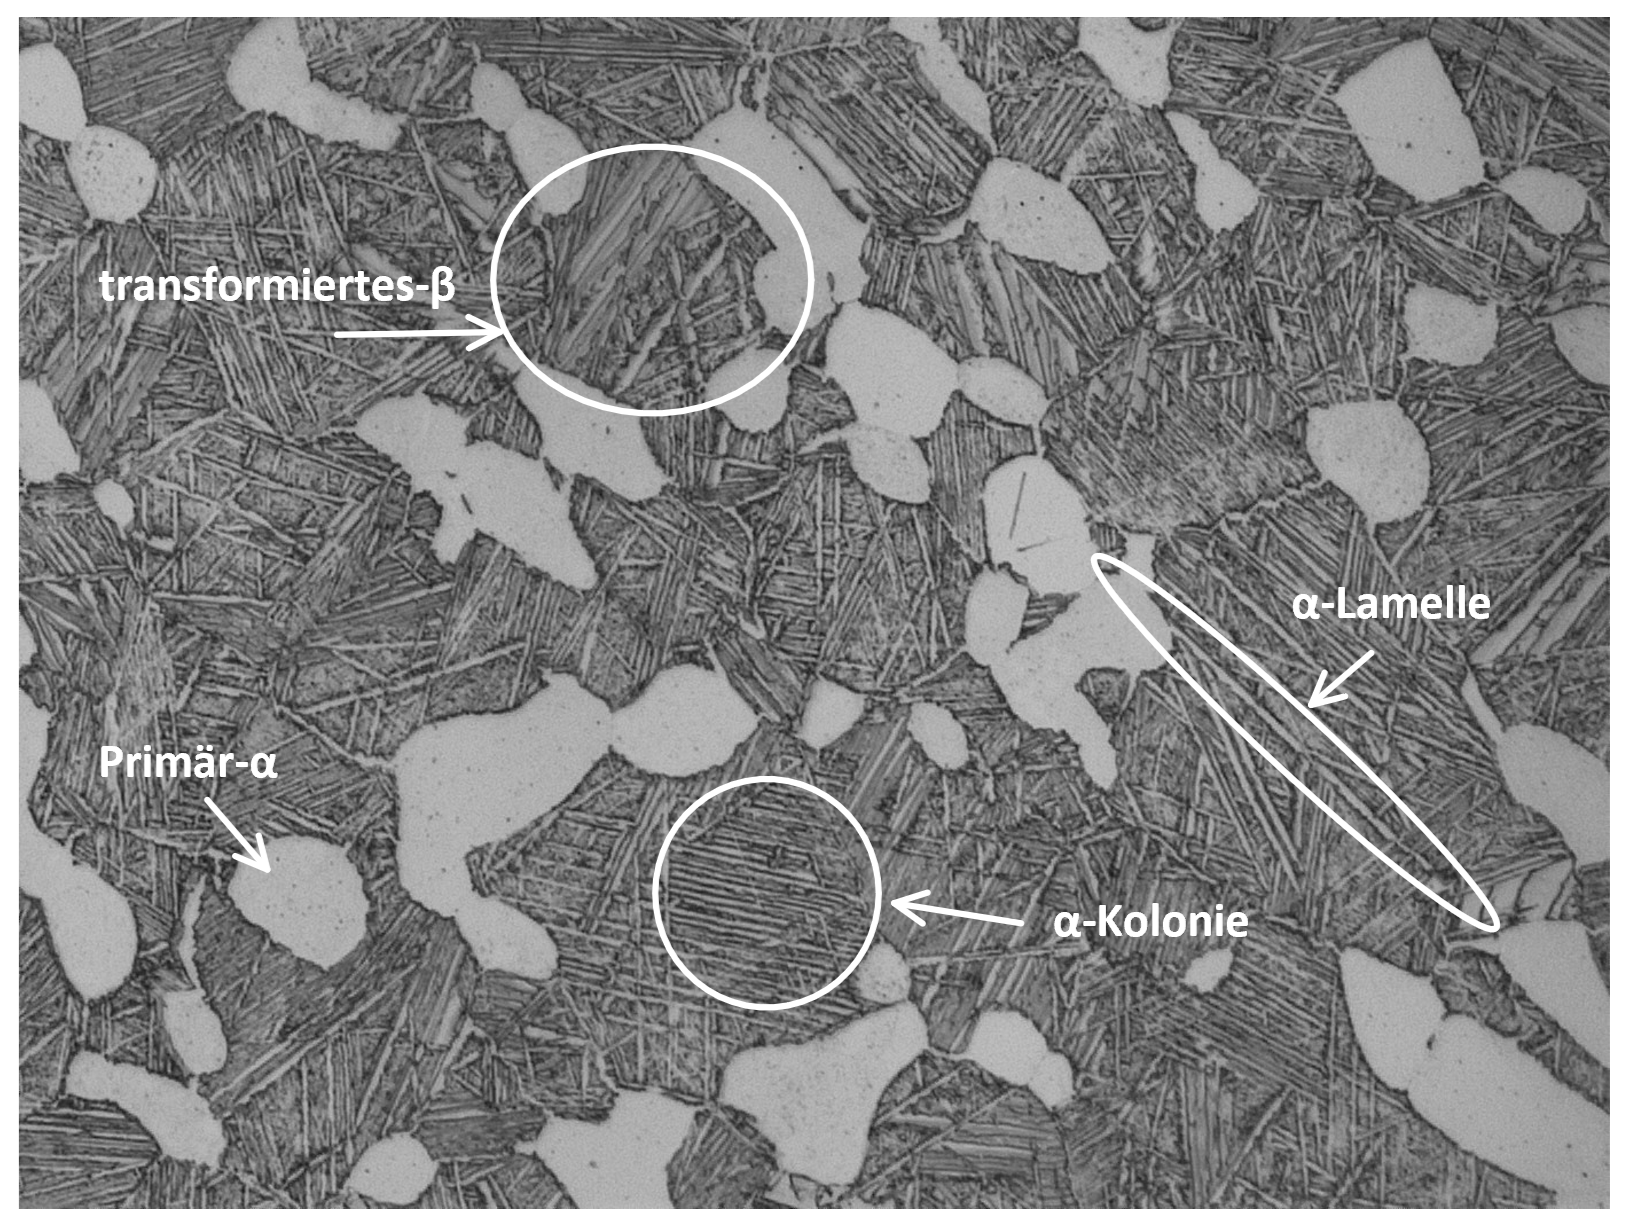
\includegraphics[width=0.6\linewidth]{./Bilder/Abbildung 20.png}
	\caption[Abbildung 20]{Gefügebestandteile in bi-modaler Mikrostruktur}
	\label{fig:abbildung-20}
\end{figure}

Die Ergebnisse der Bestimmung des $\alpha_p$-Volumenanteils mittels Bildbearbeitungsprogramm sind in Tabelle \ref{Tabelle 4} aufgeführt. Laut Lütjering und Williams liegt der optimale $\alpha_p$-Volumenanteil zur Steigerung der Zugfestigkeitswerte zwischen 10 und 20 \% \cite{Lutjering.2007}.

\begin{table}[h]
	\centering
	\begin{tabular}{|c|c|}
		\hline 
		Probe & Primär-$\alpha$ in \% \\ 
		\hline 
		AR & 62 \\ 
		\hline 
		960$^\circ$C/1h/AC & 37 \\ 
		\hline 
		975$^\circ$C/1h/AC & 26 \\ 
		\hline 
		983$^\circ$C/1h/AC & 16 \\ 
		\hline 
		990$^\circ$C/1h/AC & 9 \\ 
		\hline 
		1015$^\circ$C/30min/WQ & 0 \\ 
		\hline 
	\end{tabular} 
	\caption{$\alpha_p$-Volumenanteile der ersten Wärmebehandlungen mit einer Genauigkeit von 3\%}
	\label{Tabelle 4}
\end{table}

Die Auswertung hat ergeben, dass der angestrebte $\alpha_p$-Volumenanteil mit der Wärmebehandlung bei 983$^\circ$C für 1 h mit anschließender Luftkühlung erreicht wurde. Die vollmartensitische Probe hat wie erwartet keinen sichtbaren $\alpha_p$-Anteil aufgewiesen.


Des Weiteren wurde an der ersten Probenreihe eine Härteprüfung durchgeführt. Die Ergebnisse sind in Tabelle \ref{Tabelle 5} aufgeführt. 

\begin{table}[h]
	\centering
	\begin{tabular}{|c|c|}
		\hline 
		Probe & Härte in HV \\ 
		\hline 
		AR & 331 \\ 
		\hline 
		960$^\circ$C/1h/AC & 345 \\ 
		\hline 
		975$^\circ$C/1h/AC & 344 \\ 
		\hline 
		983$^\circ$C/1h/AC & 344 \\ 
		\hline 
		990$^\circ$C/1h/AC & 350 \\ 
		\hline 
		1015$^\circ$C/30min/WQ & 403 \\ 
		\hline 
	\end{tabular} 
	\caption{Härtewerte der ersten Probenreihe in HV}
	\label{Tabelle 5}
\end{table}

Nach der ersten Wärmebehandlung war bei den Proben mit bi-modaler Mikrostruktur eine geringe Härtesteigerung gegenüber der AR-Probe festzustellen. 
Die Probe mit vollmartensitischem Gefüge hat dagegen eine signifikante Härtesteigerung gezeigt. Dies kann durch die feinere Struktur des Martensits und dadurch erhöhte Grenzflächendichte begründet werden. Sie wurde aber im Rahmen der gewählten Strategien nicht weiter verfolgt, da bi-modale Gefüge im Hinblick auf die zu erreichende Bruchdehnung (mind. 10\%) eine bessere Basis darstellen.


\section{Diskussion der Ergebnisse (VR)}

Es zeigt sich, dass mit steigender Glühtemperatur der $\alpha_p$-Anteil geringer wird. Eine Temperatur näher an T$_{\beta}$ bedeutet einen größeren $\beta$-Phasenanteil im Gleichgewichtszustand, die bei Abkühlung teilweise in lamellares $\alpha$ transformiert. Die Glühzeit hat dabei keinen Einfluss die Mikrostruktur. Sie muss nur lang genug sein für die Bildung von isolierten, globularen $\alpha_p$-Körnern \cite{G.LutjeringJ.C.WilliamsA.Gysler.}. 
Die Werte zeigen eine Erhöhung der Härte gegenüber den AR-Proben, aber keine signifikanten Unterschiede untereinander. Die Lamellenpakete sind durch ihre feine Mikrostruktur härter gegenüber dem gröberen $\alpha_p$-Körnern, sodass ein Härteanstieg mit sinkendem $\alpha_p$-Volumenanteil zu erwarten wäre. Da die $\alpha_p$-Körner eine Wachstumsbehinderung für die transformierte $\beta$-Phase darstellen und somit die Lamellenpaketbreite begrenzen, bedeutet ein geringerer Anteil eine größere Weglänge zwischen einzelnen Körnern. Somit kommt es zu weniger Grenzflächen zwischen dem $\alpha_p$ und transformiertem $\beta$ und einer Festigkeitsabnahme. Diese zwei gegenläufigen Effekte erklären die annähernd gleichen Härtewerte für alle vier Temperaturen der Wärmebehandlung. 